\documentclass[11pt]{article}
\usepackage[a4paper, portrait, margin=1in]{geometry}
\usepackage{mathtools}
\usepackage{listings}
\usepackage[dvipsnames]{xcolor}
\usepackage{color}
\usepackage{graphicx}
\usepackage[colorlinks=true,urlcolor=blue,linkcolor=black]{hyperref}


\DeclarePairedDelimiter{\ceil}{\lceil}{\rceil}

\newcommand{\code}[1]{\lstinline[language=Java]{#1}}
\newcommand{\todo}[1]{\fcolorbox{black}{Apricot}{TODO: #1}}
\newcommand{\linkmain}[1]{\href{https://gitlab.inf.ethz.ch/pungast/asl-fall16-project/blob/master/src/main/java/asl/#1.java}{#1}}
\newcommand{\linktest}[1]{\href{https://gitlab.inf.ethz.ch/pungast/asl-fall16-project/blob/master/src/test/java/asl/#1.java}{#1}}

\newcommand{\resultsurl}[1]{\href{https://gitlab.inf.ethz.ch/pungast/asl-fall16-project/blob/master/results/#1}{gitlab.inf.ethz.ch/.../results/#1}}




\begin{document}

\title{Advanced Systems Lab (Fall'16) -- Second
Milestone}

\author{Name: \emph{Taivo Pungas}\\Legi number: \emph{15-928-336}}

\date{
\vspace{4cm}
\textbf{Grading} \\
\begin{tabular}{|c|c|}
\hline  \textbf{Section} & \textbf{Points} \\ 
\hline  1 &  \\ 
\hline  2 &  \\ 
\hline  3 &  \\ 
\hline \hline Total & \\
\hline 
\end{tabular} 
}

\maketitle

\newpage

\tableofcontents

\clearpage
% --------------------------------------------------------------------------------
% --------------------------------------------------------------------------------
\section*{Modifications to the middleware}
% --------------------------------------------------------------------------------
% --------------------------------------------------------------------------------
\addcontentsline{toc}{section}{Modifications to the middleware}

In the last milestone submission, my middleware implemented all functionality as necessary. However, the resource usage was extremely wasteful: each read thread took up nearly 100\% of the resources allocated to them and never went to a sleeping state. This caused more than 10-fold drops in performance when going from $T=1$ to $T=4$ (for $S=5$), and would have made the maximum throughput experiment useless. The changes can be seen on \href{https://gitlab.inf.ethz.ch/pungast/asl-fall16-project/commit/928e9bba132d34ecf9c00936babdd7fa2645e50f}{GitLab}.

To verify that the system is still stable, I re-ran the trace experiment. The throughput and response time are shown in Figures~\ref{fig:trace:throughput} and \ref{fig:trace:responsetime}, and are confirmed to be stable (and throughput is roughly 30\% higher). The Interactive Response Time Law also still holds (to within 0.46\%). For explanations of the figures, see Milestone 1 report.

\begin{figure}[h]
\centering
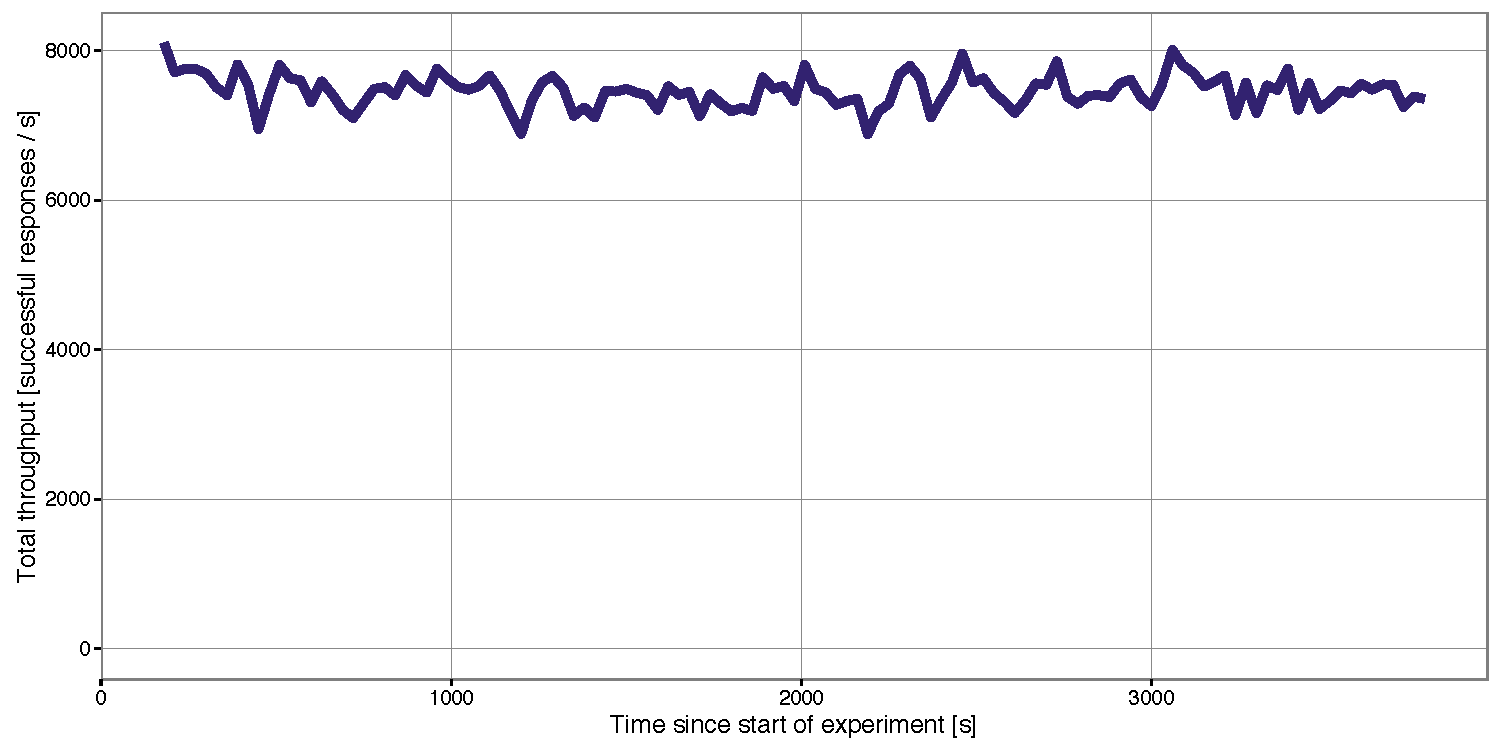
\includegraphics[width=\textwidth]{../results/trace_rep3/graphs/throughput.pdf}
\caption{Throughput trace of the middleware.}
\label{fig:trace:throughput}
\end{figure}

\begin{figure}[h]
\centering
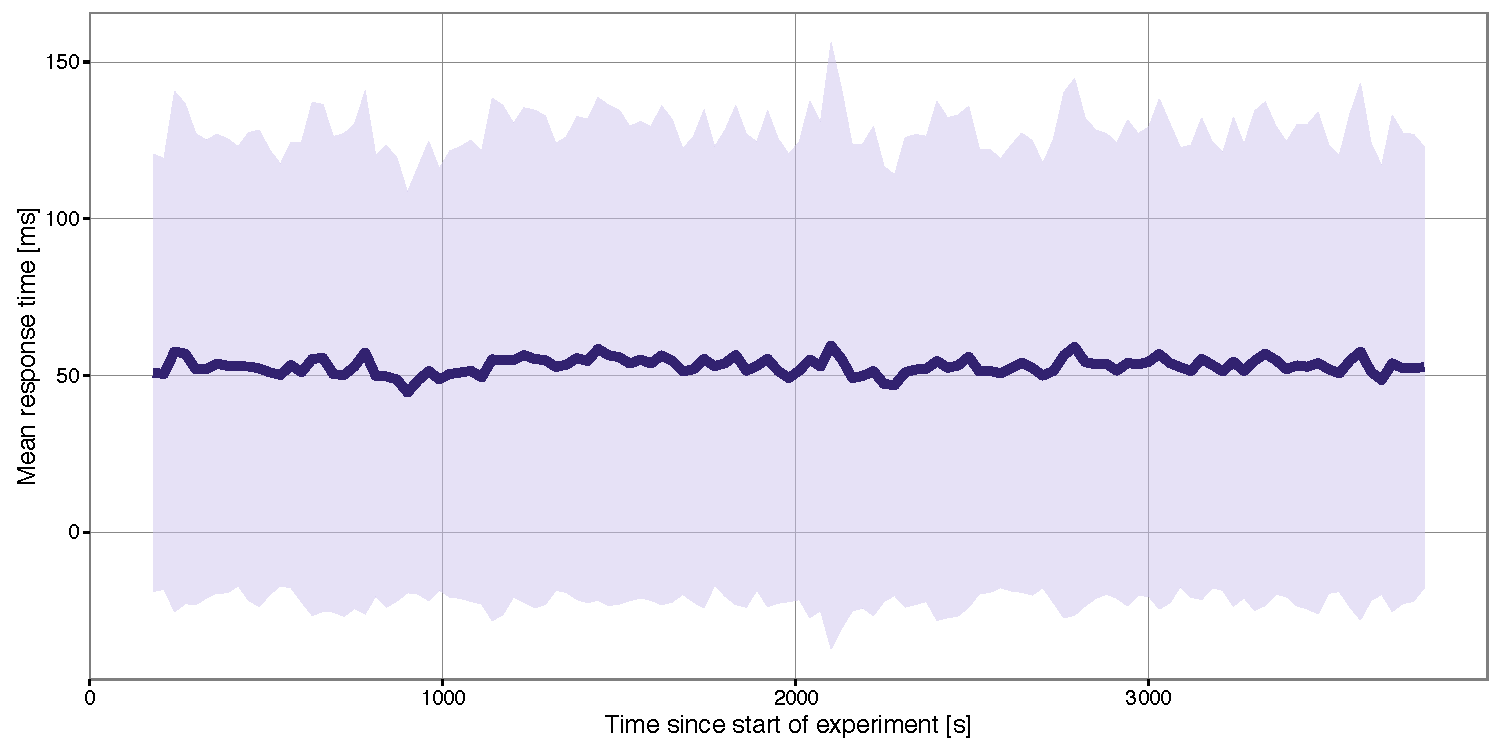
\includegraphics[width=\textwidth]{../results/trace_rep3/graphs/responsetime.pdf}
\caption{Response time trace of the middleware as measured by memaslap.}
\label{fig:trace:responsetime}
\end{figure}


% --------------------------------------------------------------------------------
% --------------------------------------------------------------------------------
\section*{Definitions and setup}
% --------------------------------------------------------------------------------
% --------------------------------------------------------------------------------
\addcontentsline{toc}{section}{Definitions and setup}

In all experiments, the following definitions hold.

\begin{itemize}
\item The \emph{system under test} (SUT) is the middleware together with the connected memcached servers, running on Ubuntu virtual machines in the Azure cloud.
\item \emph{Throughput} is the number of requests the SUT successfully responds to, per unit of time, as measured by memaslap.
\item \emph{Response time (memaslap)} is the time from sending to receiving the request to the SUT including any network latencies, as measured by the client (memaslap).
\item \emph{Response time (middleware)} is the time from receiving the request in the middleware ($t_{created}$) to returning it to the client ($t_{returned}$), as measured by the middleware.
\end{itemize}

In all experiments, the following holds about the experimental setup:
\begin{itemize}
\item The middleware was run on Basic A4 instances, and both memaslap and memcached were run on Basic A2 instances.
\item The first 2 and last 2 minutes of each experiment were discarded from analyses as warm-up and cool-down time.
\item The request sampling rate for logging is set to $\frac{1}{100}$ in throughput experiments (Section~\ref{sec:exp1}) and $\frac{1}{10}$ in replication and write proportion experiments (Sections~\ref{sec:exp2} and \ref{sec:exp3}).
\item Response times inside the middleware were measured with a 1 millisecond accuracy.
\item The system is closed because memaslap clients wait for a response before sending a new request.
\end{itemize}


\clearpage
% --------------------------------------------------------------------------------
% --------------------------------------------------------------------------------
\section{Maximum Throughput}
% --------------------------------------------------------------------------------
% --------------------------------------------------------------------------------
\label{sec:exp1}

\subsection{Experimental question}

In this section, I will run experiments to find out a) the maximum throughput of the SUT, b) the number of read threads ($T$) in the middleware that achieves this c) the number of virtual clients ($C$) that achieves this.

To this end, I will measure throughput as a function of $T$ and $C$, in 10-second time windows. I will find the maximum sustained throughput of the SUT, i.e. the throughput at which the response time does not increase rapidly with additional clients. For each parameter combination, I will run experiments until the 95\% confidence interval (calculated using a two-sided t-test) lies within 5\% of the mean throughput.

\subsection{Hypothesis}

I approximate that the maximum throughput will be 17200 requests per second using 50 read threads in the middleware at a load of 192 to 550 clients.

\paragraph{Number of threads} 
Given that requests spend most of their time ($\sim90\%$ in the trace experiment) waiting in the queue, increasing $T$ will increase throughput. If we reduce the queueing time by a factor of 10, it will no longer be the bottleneck (then waiting for memcached's response -- which takes $\sim9\%$ of response time in the trace experiment -- becomes the bottleneck). Assuming the time spent in the queue scales linearly with the number of read threads, we should increase $T$ 10-fold, i.e. $T=50$ maximises throughput.

\paragraph{Number of clients}
Throughput will be maximised at roughly 110 virtual clients per memcached server, so 550 virtual clients in total. This is based on the fact that in the Milestone 1 baseline experiment, the throughput of a single memcached server without middleware saturated at around 110 virtual clients. It is likely to be an overestimate since the SUT here has an additional part (the middleware) and the baseline experiment did not measure sustained throughput, but 550 clients is a reasonable upper bound. As a lower bound we can use the number of clients in the trace experiment: $3 \cdot 64=192$.

\paragraph{Throughput}
Since in the trace experiment, the throughput was roughly 10300 requests per second, we have a lower bound for the expected throughput. Naively assuming that the throughput of GET requests scales linearly with the number of servers $S$ would yield an expected throughput of $\frac{5}{3} \cdot 10300 = 17200$ requests per second. However, this does not take into account that we will also increase the number of threads (from $T=5$ in the trace experiment). Thus I expect the maximum sustained throughput to be definitely more than 10300 requests per second, and likely to be more than 17200 requests per second.

I predict that the graph of throughput as a function of the number of clients will be similar to Figure~\ref{fig:exp1:hyp:throughput}: rapidly increasing at first, then reaching the knee after which throughput growth is much slower, and then saturating. After saturation, the throughput may fall due to unexpected behaviour in the middleware.

\begin{figure}[h]
\centering
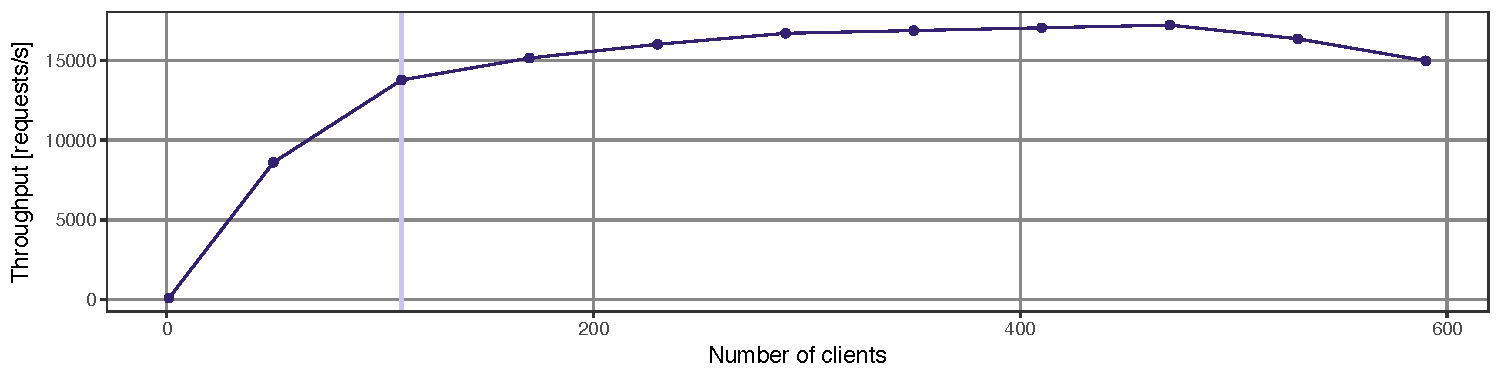
\includegraphics[width=\textwidth]{figures/hypothesis_throughput.pdf}
\caption{Expected graph of throughput as a function of number of clients (for the optimal value of $T$). The vertical line shows the optimal number of clients.}
\label{fig:exp1:hyp:throughput}
\end{figure}

\subsection{Experiments}
\begin{center}
\small{
\smallskip
\begin{tabular}{|c|c|}
\hline Number of servers & 5 \\ 
\hline Number of client machines & $\in \{1, 3\}$ \\ 
\hline Virtual clients & $\in \{1, 36, 72, 144, 180, 216, 288, 360, 432, 504, 576, 648\}$ \\ 
\hline Workload & Key 16B, Value 128B, Writes 0\% \\
\hline Middleware: replication factor & 1 \\ 
\hline Middleware: read threads & $\in\{1, 16, 32, 64\}$ \\ 
\hline Runtime x repetitions & at least 6min x 1; more in some cases \\ 
\hline Log files & throughput-C*-T*-r* \\
\hline 
\end{tabular} }
\end{center}

Three client machines were used for all experiments, except for the 1-client experiment, where only one machine was used.

The values of $T$ to test were $T=1$ as the lowest possible value, and then from $T=16$ in multiplicative steps of 2. The reason for the small number of tested values of $T$ is pragmatic: it doesn't require hundreds of experiments and at the same time gives a reasonable approximation of the optimal $T$.

Some parameter combinations did not yield the required confidence interval in the first 6-minute repetition of the experiment. When that was the case, I re-ran the experiment (in some cases for a longer time), thus producing more datapoints and decreasing the confidence interval.

\subsection{Results}
Reporting experiment results.

\begin{figure}[h]
\centering
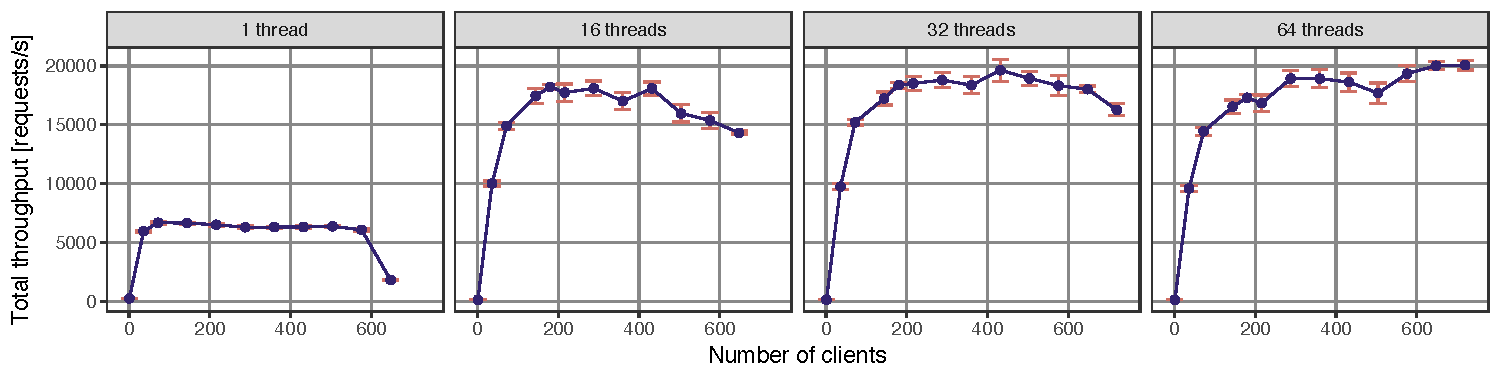
\includegraphics[width=\textwidth]{../results/throughput/graphs/tp_vs_clients.pdf}
\caption{Throughput as a function of $C$ for different values of $T$. Errorbars show the 95\% confidence interval around the mean value which is shown with points connected by lines.}
\label{fig:exp1:res:throughput}
\end{figure}

\begin{figure}[h]
\centering
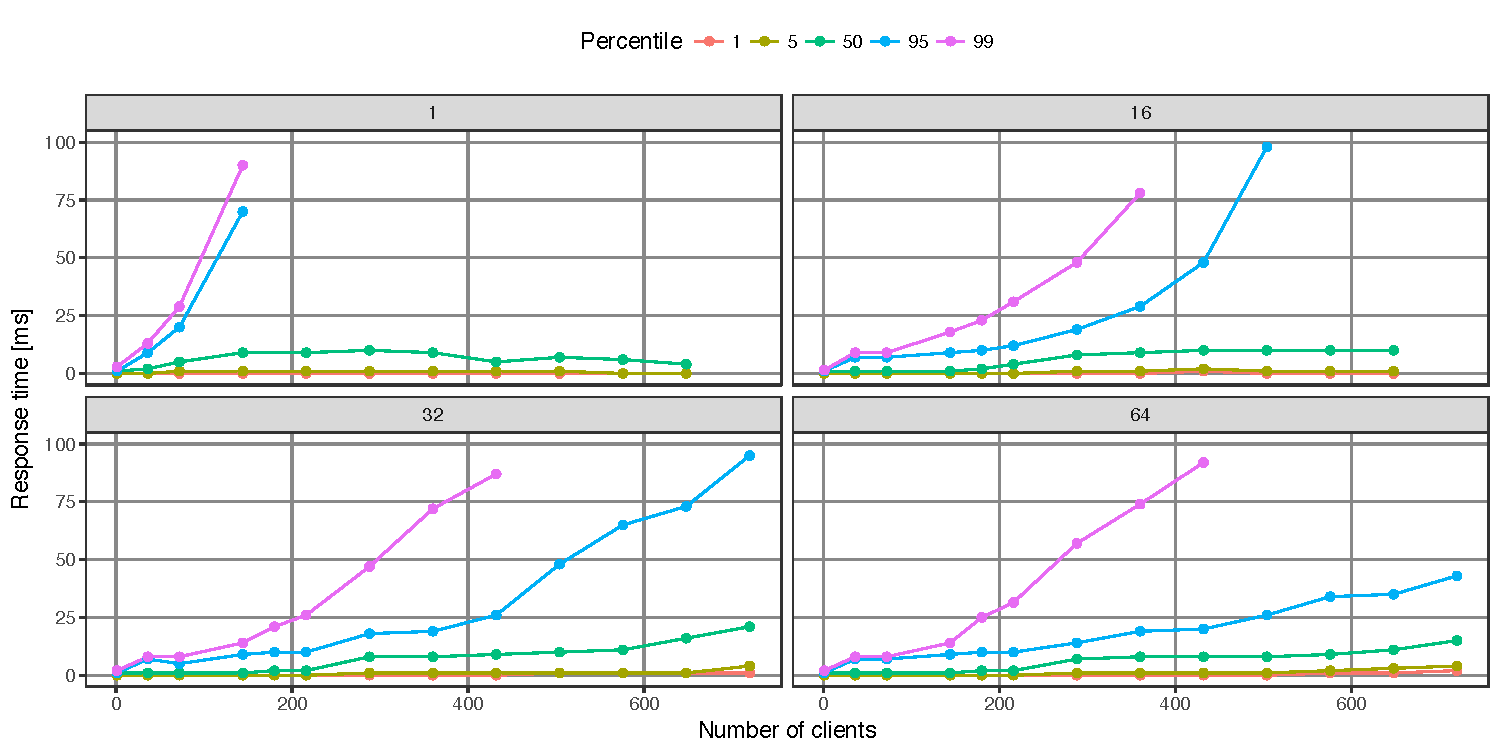
\includegraphics[width=\textwidth]{../results/throughput/graphs/response_time_vs_clients.pdf}
\caption{The 1\%, 5\%, 50\%, 95\% and 99\% percentiles of the response time (middleware) distribution, as a function of $C$ for different values of $T$. Values above 100ms are not shown.}
\label{fig:exp1:res:responsetime}
\end{figure}

\begin{figure}[h]
\centering
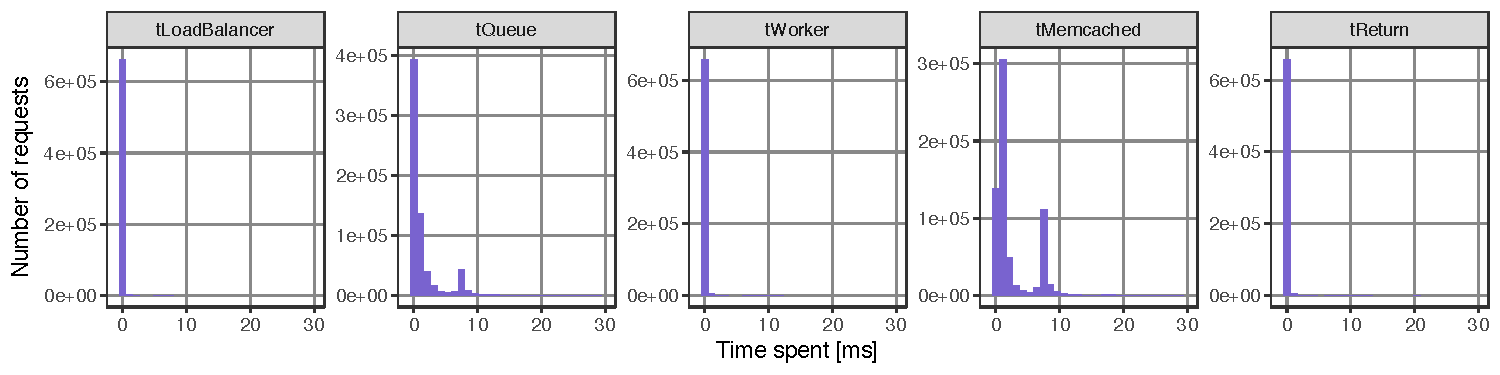
\includegraphics[width=\textwidth]{../results/throughput/graphs/response_time_breakdown.pdf}
\caption{The distribution of times that GET requests spend in different parts of SUT. Note the time axis only shows values up to 50ms (which contains the majority of datapoints) cut off at 50ms. Measurements were made with an accuracy of 1ms.}
\label{fig:exp1:res:breakdown}
\end{figure}

\begin{tabular}{|c|c|c|r|}
\hline \textbf{Name} & \textbf{Begin timestamp} & \textbf{End timestamp} & \textbf{Mean [ms]} \\
\hline tLoadBalancer & $t_{created}$ & $t_{enqueued}$ & 0.0043 \\
\hline tQueue & $t_{enqueued}$ & $t_{dequeued}$ & 1.40 \\
\hline tWorker & $t_{dequeued}$ & $t_{forwarded}$ & 0.0191 \\
\hline tMemcached & $t_{forwarded}$ & $t_{received}$ & 2.85 \\
\hline tReturn & $t_{received}$ & $t_{returned}$ & 0.0221 \\
\end{tabular}


\todo{Comparison of hypothesis and experiment results.}

\todo{Mention the table of mean times and Figure~\ref{fig:exp1:res:breakdown}.}

Figure~\ref{fig:exp1:res:throughput} shows that the highest throughput was achieved using $T=64$ at 720 clients (20100 requests/s), followed by $T=64$ at 648 clients (20000 requests/s) and $T=32$ at 432 clients (19600 requests/s). However, since we are trying to maximise sustained throughput, we also need to look at the response times.

Figure~\ref{fig:exp1:res:responsetime} shows the percentiles of the response time distribution for each parameter set. It is apparent that for all values of $T > 1$, both the median response time (green line) and 95\% quantile (blue line) increase significantly after 216 clients. For this reason, we will exclude all values of $T > 216$ from consideration as unsustainable. Of the remaining setups, the highest throughput is achieved both by 180 and 216 clients at $T=32$. Thus we pick the one with the lower number of clients -- 180 clients and 32 threads -- as the configuration we will declare optimal at a throughput of 18400 requests per second.




\clearpage
% --------------------------------------------------------------------------------
% --------------------------------------------------------------------------------
\section{Effect of Replication}
% --------------------------------------------------------------------------------
% --------------------------------------------------------------------------------
\label{sec:exp2}

\subsection{Experimental question}

In this section, I will run experiments to find out how the response time of the SUT depends on the number of servers $S$ and replication factor $R$. Additionally, I will investigate whether gets and sets are differently affected by these parameters. Finally, I will find out which operations become more time-consuming as these parameters change.

To this end, I will measure response time (for every 10th request) as a function of $S$ and $R$, and measure how long requests spend in each part of the SUT (based on the timestamps defined in Milestone 1). For each parameter combination, I will run experiments until the 95\% confidence interval (calculated using a two-sided t-test) lies within 5\% of the mean response time.

\subsection{Hypothesis}

I predict the following.

\paragraph{Get and set requests}
Get and set requests will not be impacted the same way by different setups.

Get requests will be processed faster as we increase $S$ because the same load will be distributed across more threads. Increasing $R$ will have no effect on get requests because replication is only done for set requests (there may be secondary effects due to e.g. write threads requiring more CPU time, but this should be negligible).

Set requests will be strongly affected by $R$. If $R=1$, set requests will be processed faster for higher $S$ because each request is only written to one server, and for a higher $S$ the same load is distirbuted across more write threads. However, if $R>1$, response time of sets increases due to two factors: a) the request is written serially to $R$ servers, and b) not all $R$ responses are received at the same time. Assuming a) is negligible compared to b), we will observe an increase in the mean response time.

All of this is summarised in Figure~\ref{fig:exp2:hyp:replication}. For get requests, response time will be independent of $R$ for any fixed $S$. For set requests, response time increases linearly with increasing $R$, and the slope increases with $S$.

\begin{figure}[h]
\centering
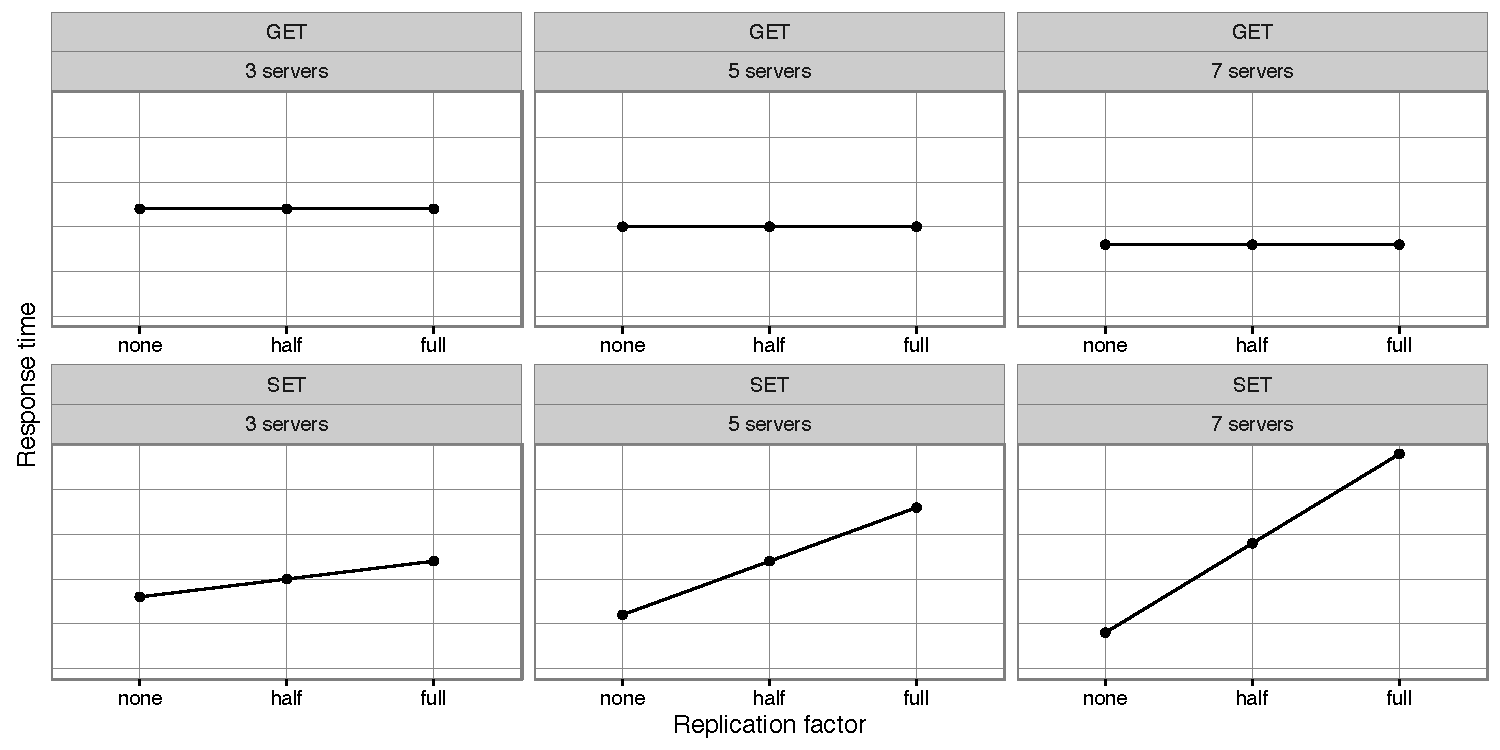
\includegraphics[width=\textwidth]{figures/hypothesis_replication.pdf}
\caption{Expected response times of SUT. The vertical (time) axis has an arbitrary but fixed scale for all plots in the top row, and a different but also fixed scale for the bottom row.}
\label{fig:exp2:hyp:replication}
\end{figure}

\paragraph{Relative cost of operations}
As explained previously, more replication means that the middleware needs to send each set request to more servers and wait for more answers. Thus, as $R$ increases, tMemcached will increase. Since each set request takes longer to process, this means that tQueue will increase as well. I also predict that the relative cost of get operations will not change.


\paragraph{Scalability}

In an ideal system, a) there would be enough resources to concurrently run all threads; b) all memcached servers would take an equal and constant amount of time to respond; c) there would be no network latencies; d) dequeueing would take constant time.

For get requests, the ideal system would have linear speed-up (assuming the load balancer does not become a bottleneck). I predict that the SUT will have sublinear speed-up because the response time also includes network latency -- a term that is not dependent on $S$: $response \; time = const. + \frac{const.}{S}$. In addition, since threads compete for resources in the SUT, the speed-up will be even lower than what's predicted by the formula above.

\subsection{Experiments}
\begin{center}
\small{
\smallskip
\begin{tabular}{|c|c|}
\hline Number of servers & $\in \{3, 5, 7\}$ \\ 
\hline Number of client machines & 3 \\ 
\hline Virtual clients & 180 \\ 
\hline Workload & Key 16B, Value 128B, Writes 5\% \\
\hline Middleware: replication factor & $\in \{1, ceil(S/2), S\}$ \\ 
\hline Middleware: read threads & 32 \\ 
\hline Runtime x repetitions & 6min x 1 \\ 
\hline Log files & replication-S*-R*-r* \\
\hline 
\end{tabular} }
\end{center}

\subsection{Results}
Reporting experiment results. Comparison of hypothesis and experiment results.
How does the scalability of your system compare to that of an ideal implementation?

\todo{table: y axis is S, x axis is R}; in each cell is corresponding response time -- separately for gets and sets?

\todo{analyse relative cost of operations} (also add in graphs where necessary)

\begin{figure}[h]
\centering
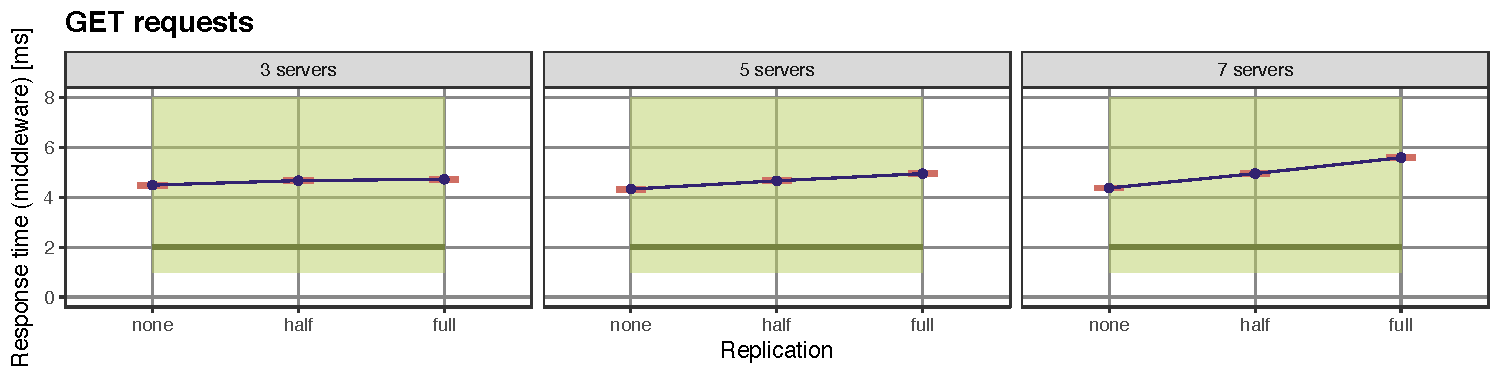
\includegraphics[width=\textwidth]{../results/replication/graphs/response_time_vs_replication_get.pdf}
\caption{Response time (middleware) to \textbf{GET} requests as a function of $R$, for different values of $S$. The line and points show the mean response time; red errorbars show the 95\% confidence interval in a double-tailed t-test; the green area shows the 25\% (bottom edge) and 75\% (top edge) quantiles of response times.}
\label{fig:exp2:res:replication:get}
\end{figure}

\begin{figure}[h]
\centering
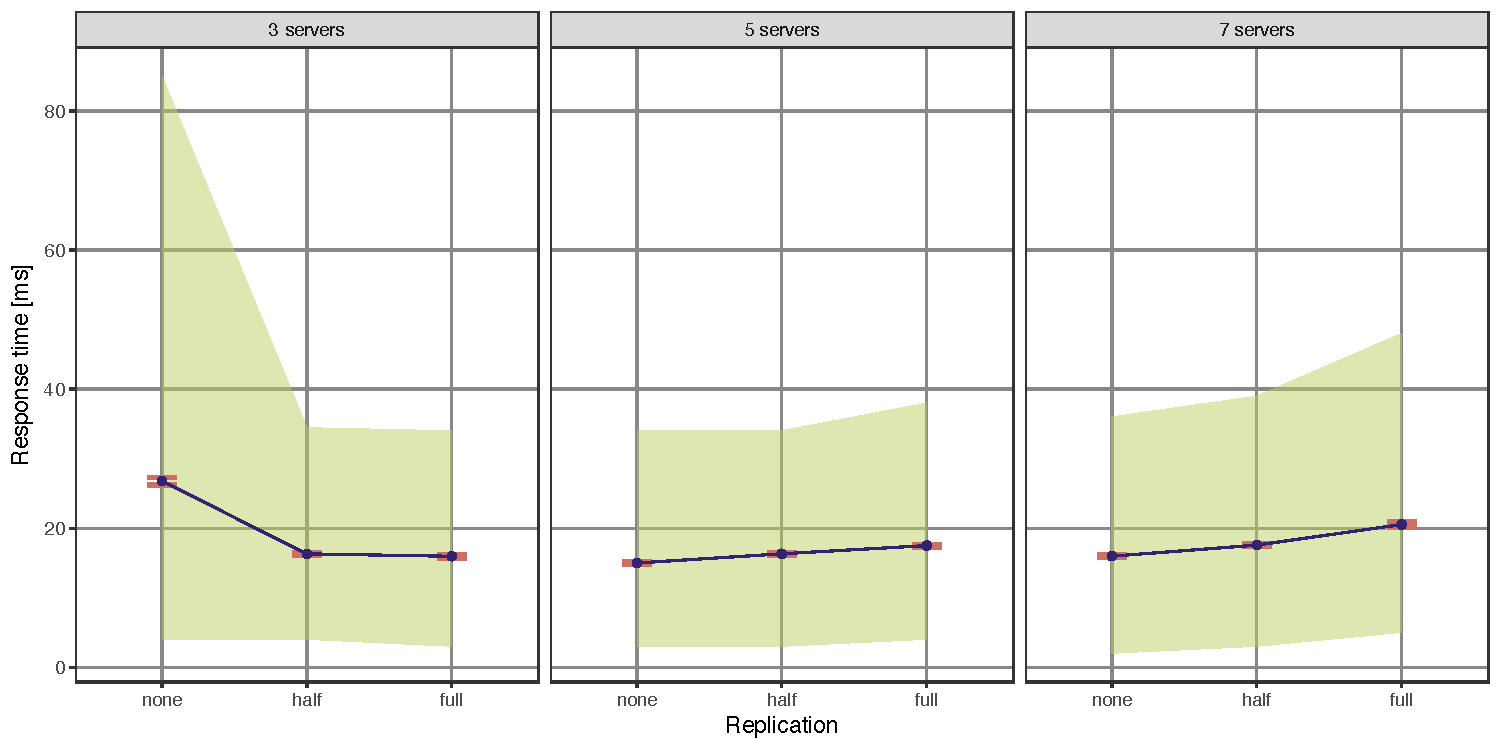
\includegraphics[width=\textwidth]{../results/replication/graphs/response_time_vs_replication_set.pdf}
\caption{Response time (middleware) to \textbf{SET} requests as a function of $R$, for different values of $S$. The line and points show the mean response time; red errorbars show the 95\% confidence interval in a double-tailed t-test; the green area shows the 25\% (bottom edge) and 75\% (top edge) quantiles of response times.}
\label{fig:exp2:res:replication:set}
\end{figure}

\begin{figure}[h]
\centering
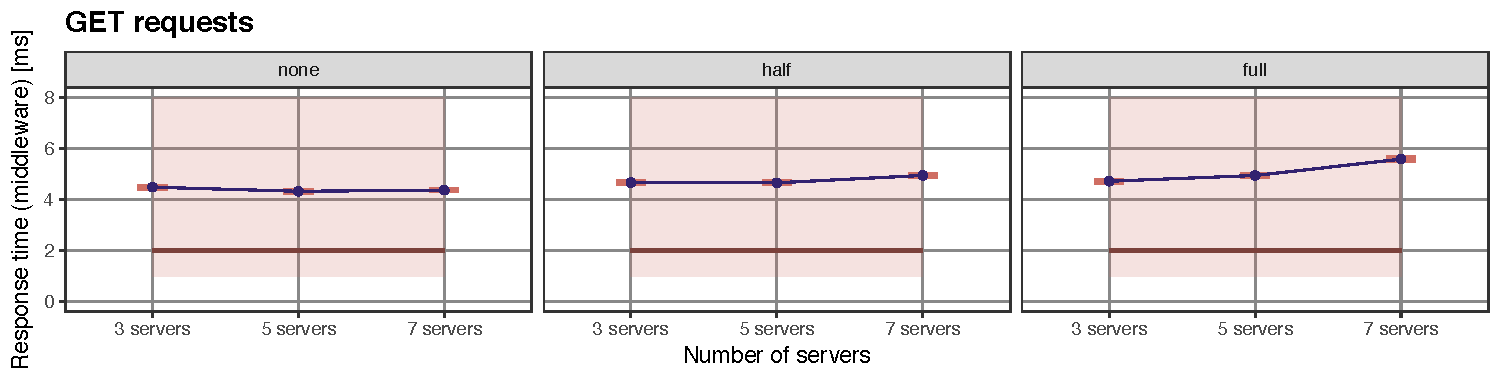
\includegraphics[width=\textwidth]{../results/replication/graphs/response_time_vs_servers_get.pdf}
\caption{Response time (middleware) to \textbf{GET} requests as a function of $S$, for different values of $R$. The line and points show the mean response time; red errorbars show the 95\% confidence interval in a double-tailed t-test; the light red area shows the 25\% (bottom edge) and 75\% (top edge) quantiles of response times.}
\label{fig:exp2:res:servers:get}
\end{figure}
 

\begin{figure}[h]
\centering
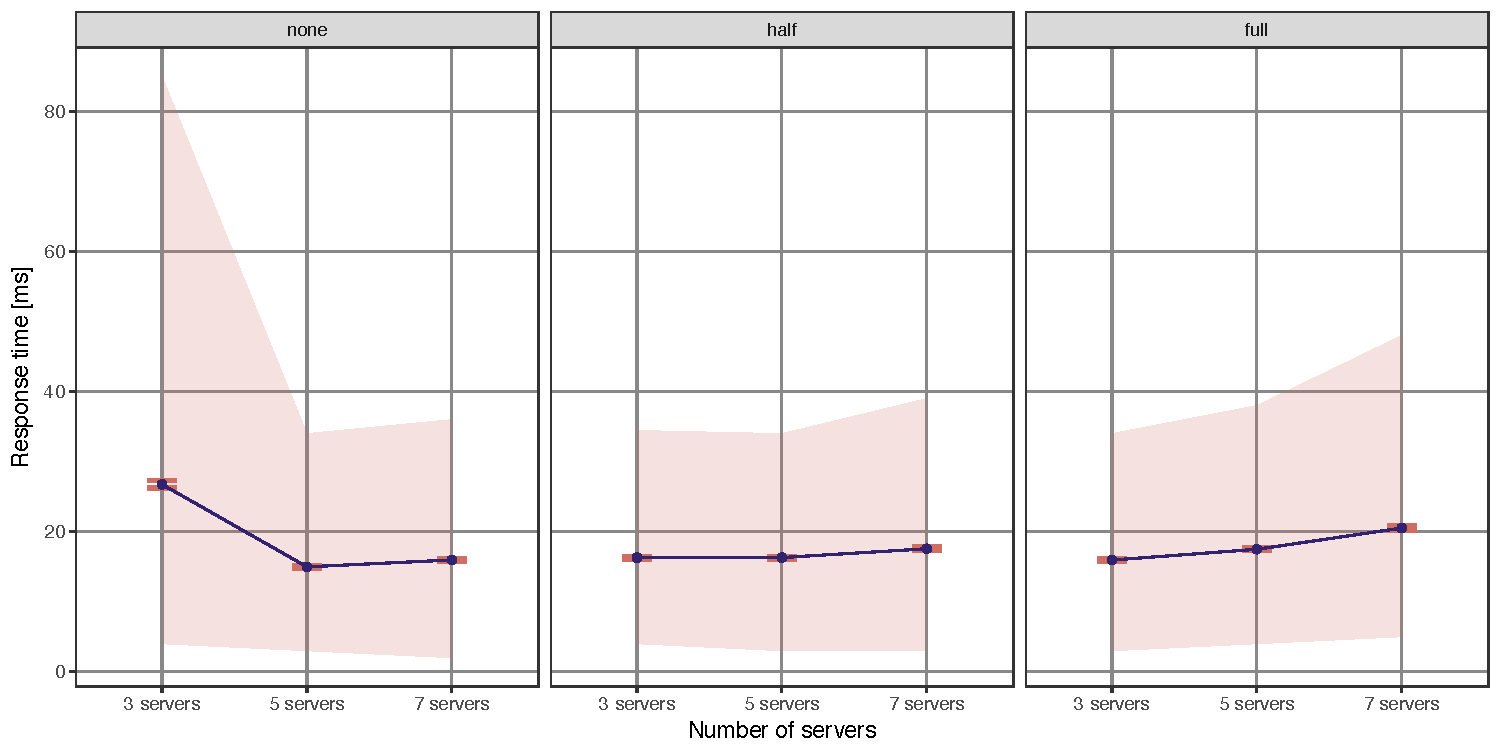
\includegraphics[width=\textwidth]{../results/replication/graphs/response_time_vs_servers_set.pdf}
\caption{Response time (middleware) to \textbf{SET} requests as a function of $S$, for different values of $R$. The line and points show the mean response time; red errorbars show the 95\% confidence interval in a double-tailed t-test; the light red area shows the 25\% (bottom edge) and 75\% (top edge) quantiles of response times.}
\label{fig:exp2:res:servers:set}
\end{figure}

\begin{figure}[h]
\centering
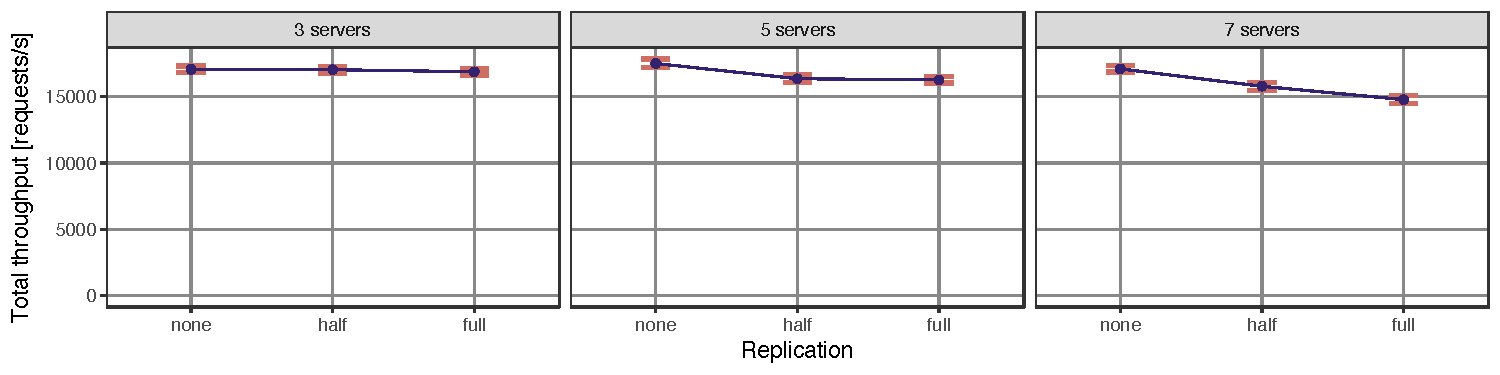
\includegraphics[width=\textwidth]{../results/replication/graphs/tp_vs_replication_all.pdf}
\caption{Throughput of SUT as a function of $R$, for different values of $S$. The line and points show the mean throughput; red errorbars show the 95\% confidence interval over 10-second samples in a double-tailed t-test.}
\label{fig:exp2:res:throughput}
\end{figure}
 

 \clearpage
% --------------------------------------------------------------------------------
% --------------------------------------------------------------------------------
\section{Effect of Writes}
% --------------------------------------------------------------------------------
% --------------------------------------------------------------------------------
\label{sec:exp3}

\subsection{Experimental question}

In this section, I will run experiments to find out how the response time and throughput of the SUT depend on the proportion of write requests, $W$. I will investigate this relationship for different values of $S$ and $R \in {1, S}$. Finally, I will find out the main reason for the reduced performance.

To this end, I will measure throughput (in 10-second time windows) and response time (for every 10th request) as a function of $W$, $S$ and $R$, and measure how long requests spend in each part of the SUT (based on the timestamps defined in Milestone 1). For each parameter combination, I will run experiments until the 95\% confidence interval (calculated using a two-sided t-test) lies within 5\% of the mean throughput.

\subsection{Hypothesis}

I predict the following.

\paragraph{Performance impact}
Increasing $W$ will decrease throughput and increase mean response time for any combination of $S$ and $R$ because write requests take longer to process. Fully replicated setups ($R=S$) will suffer a larger performance decrease than setups with no replication ($R=1$) because in the case of full replication, WriteWorkers do more work for each write request (i.e. the response time of each write request will be higher).

The setups with $S=3$ servers will suffer the largest relative performance decrease (compared to $S > 3$) because there are fewer WriteWorkers dealing with the same load of write requests, which in turn increases the queue wait time $tQueue$.

\subsection{Experiments}
\begin{center}
\small{
\smallskip
\begin{tabular}{|c|c|}
\hline Number of servers & $\in \{3, 5, 7\}$ \\ 
\hline Number of client machines & 3 \\ 
\hline Virtual clients & 180 \\ 
\hline Workload & Key 16B, Value 128B, Writes $\in \{1\%, 4\%, 7\%, 10\%\}$ \\
\hline Middleware: replication factor & $\in \{1, S\}$ \\ 
\hline Middleware: read threads & 32 \\ 
\hline Runtime x repetitions & 8min x 1; more in one case \\ 
\hline Log files & writes-S*-R*-W*-r* \\
\hline 
\end{tabular} }
\end{center}

One parameter combination ($S=3, R=3, W=1\%$) did not yield the required confidence interval in the first repetition of the experiment so I re-ran the experiment thus producing more datapoints and decreasing the confidence interval.

\subsection{Results}
Reporting experiment results. Comparison of hypothesis and experiment results.

\todo{Analyse results}

\begin{figure}[h]
\centering
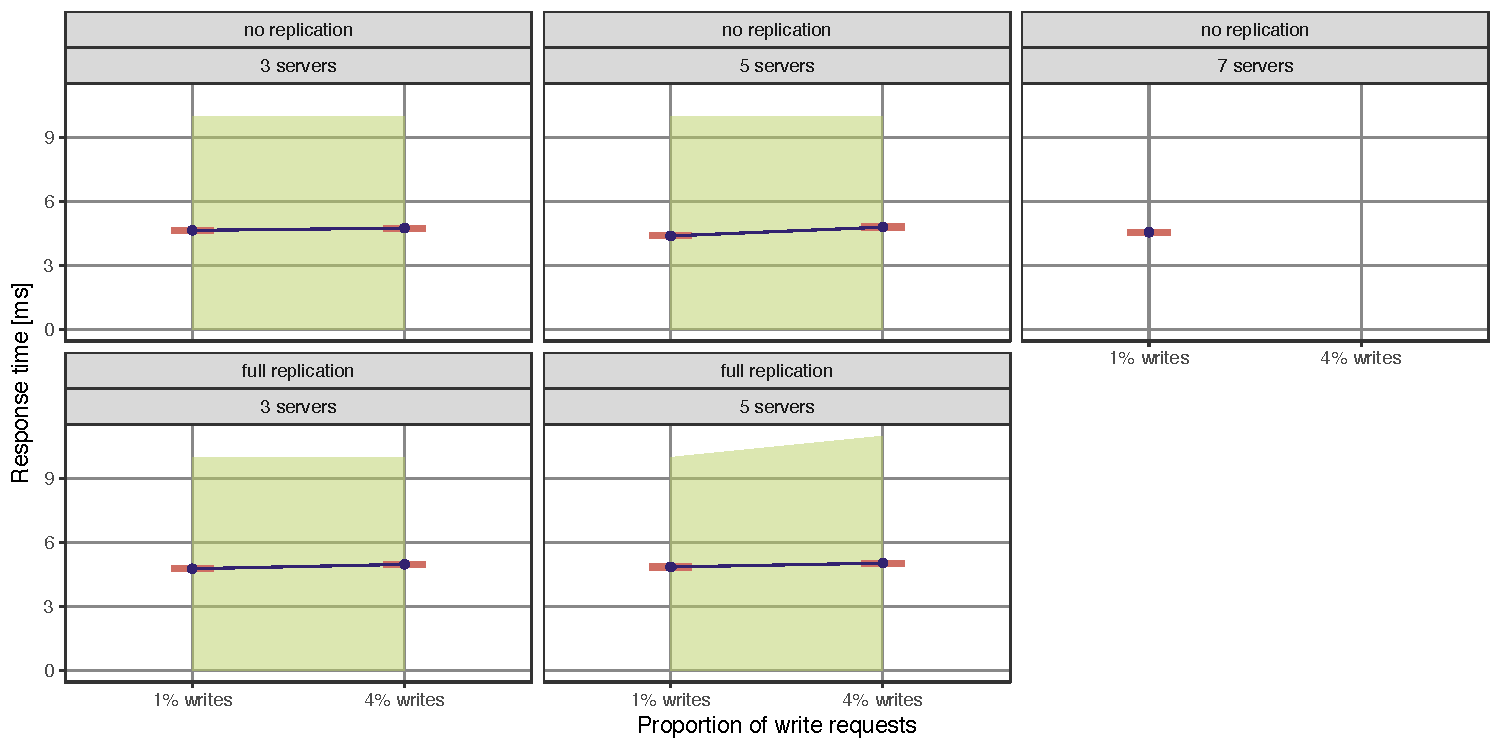
\includegraphics[width=\textwidth]{../results/writes/graphs/response_time_vs_writes_get.pdf}
\caption{Response time (middleware) to \textbf{GET} requests as a function of $W$, for different values of $S$ and $R$. The line and points show the mean response time; red errorbars show the 95\% confidence interval in a double-tailed t-test; the green area shows the 25\% (bottom edge) and 75\% (top edge) quantiles of response times.}
\label{fig:exp3:res:responsetime:get}
\end{figure}

\begin{figure}[h]
\centering
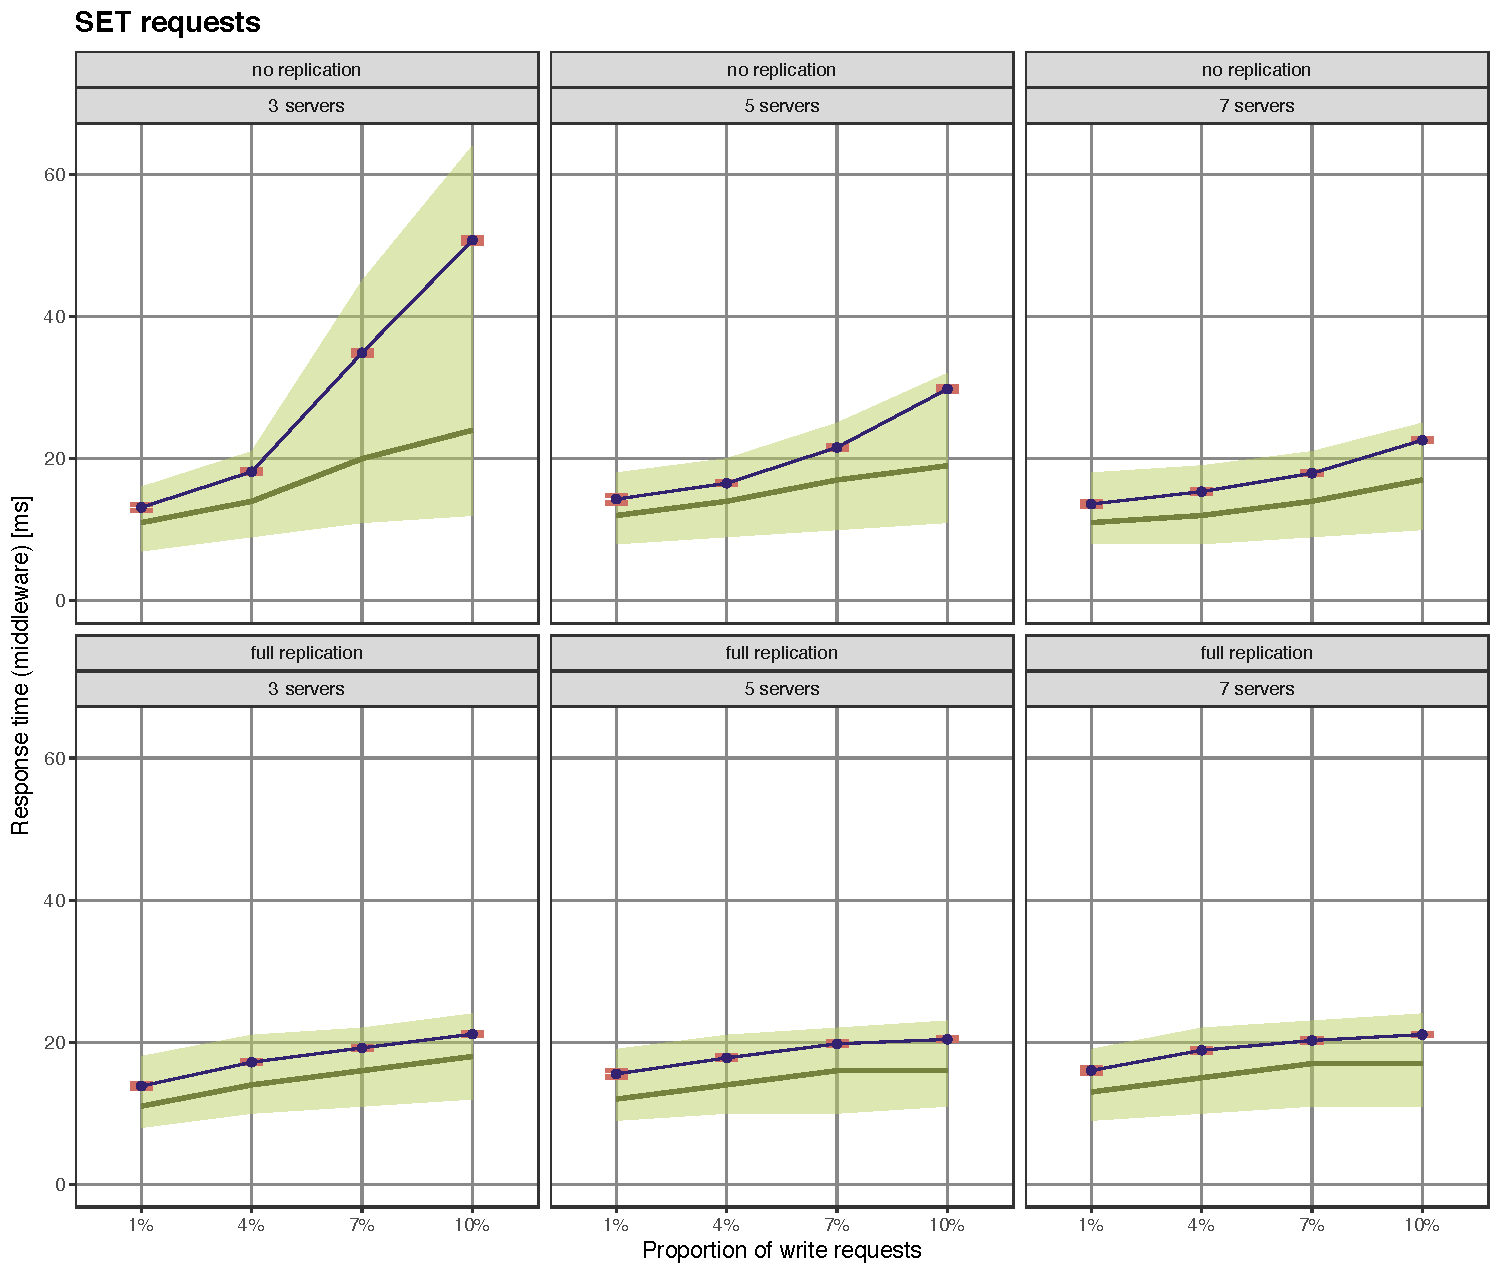
\includegraphics[width=\textwidth]{../results/writes/graphs/response_time_vs_writes_set.pdf}
\caption{Response time (middleware) to \textbf{SET} requests as a function of $W$, for different values of $S$ and $R$. The line and points show the mean response time; red errorbars show the 95\% confidence interval in a double-tailed t-test; the green area shows the 25\% (bottom edge) and 75\% (top edge) quantiles of response times.}
\label{fig:exp3:res:responsetime:set}
\end{figure}

\begin{figure}[h]
\centering
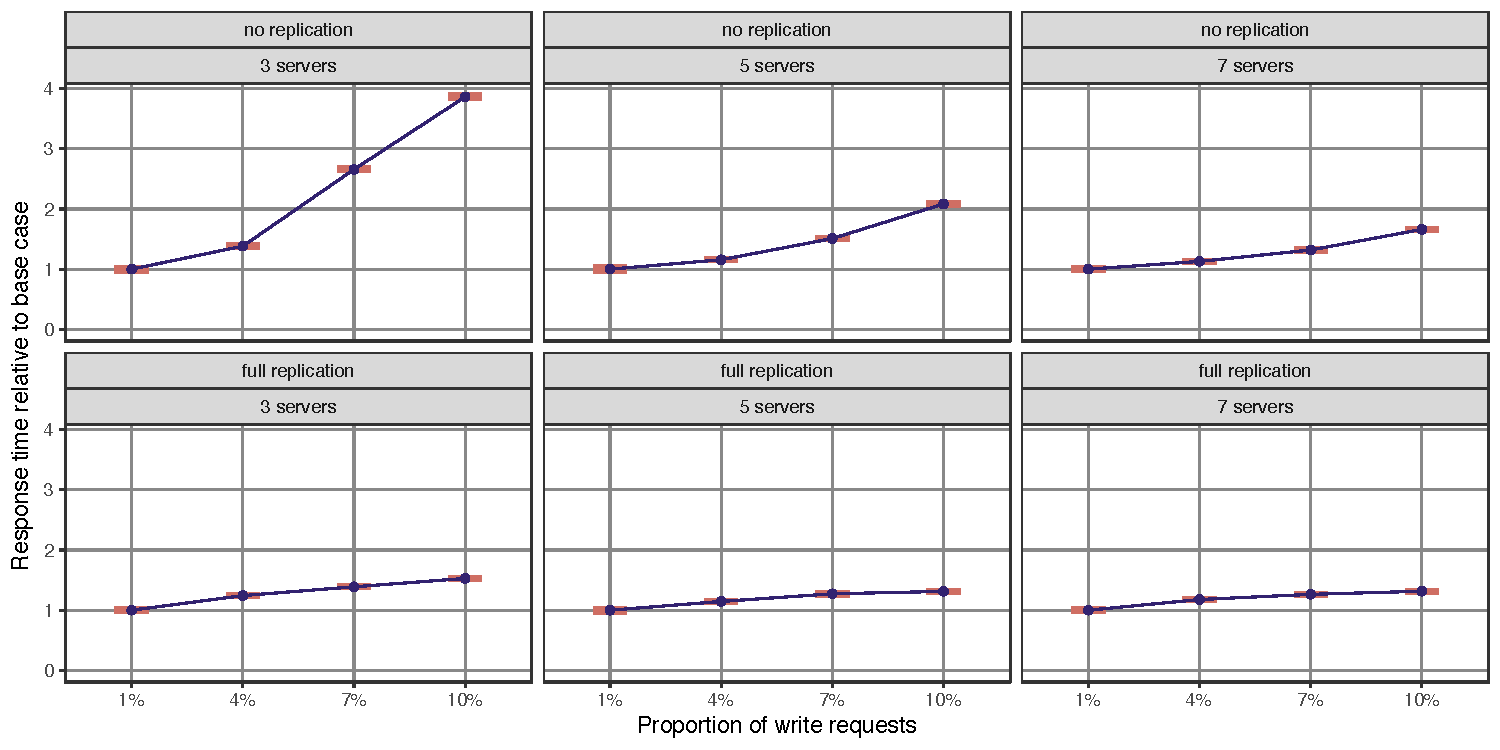
\includegraphics[width=\textwidth]{../results/writes/graphs/relative_performance_set.pdf}
\caption{Relative performance of SET requests for different values of $S$ and $R$: the response time (middleware) of each setup relative to (divided by) the response time in the base case. The base case is taken to be $W=1\%$ for each combination of $R$ and $S$.
The line and points show the mean response time; red errorbars show the 95\% confidence interval in a double-tailed t-test.}
\label{fig:exp3:res:relative:set}
\end{figure}

\begin{figure}[h]
\centering
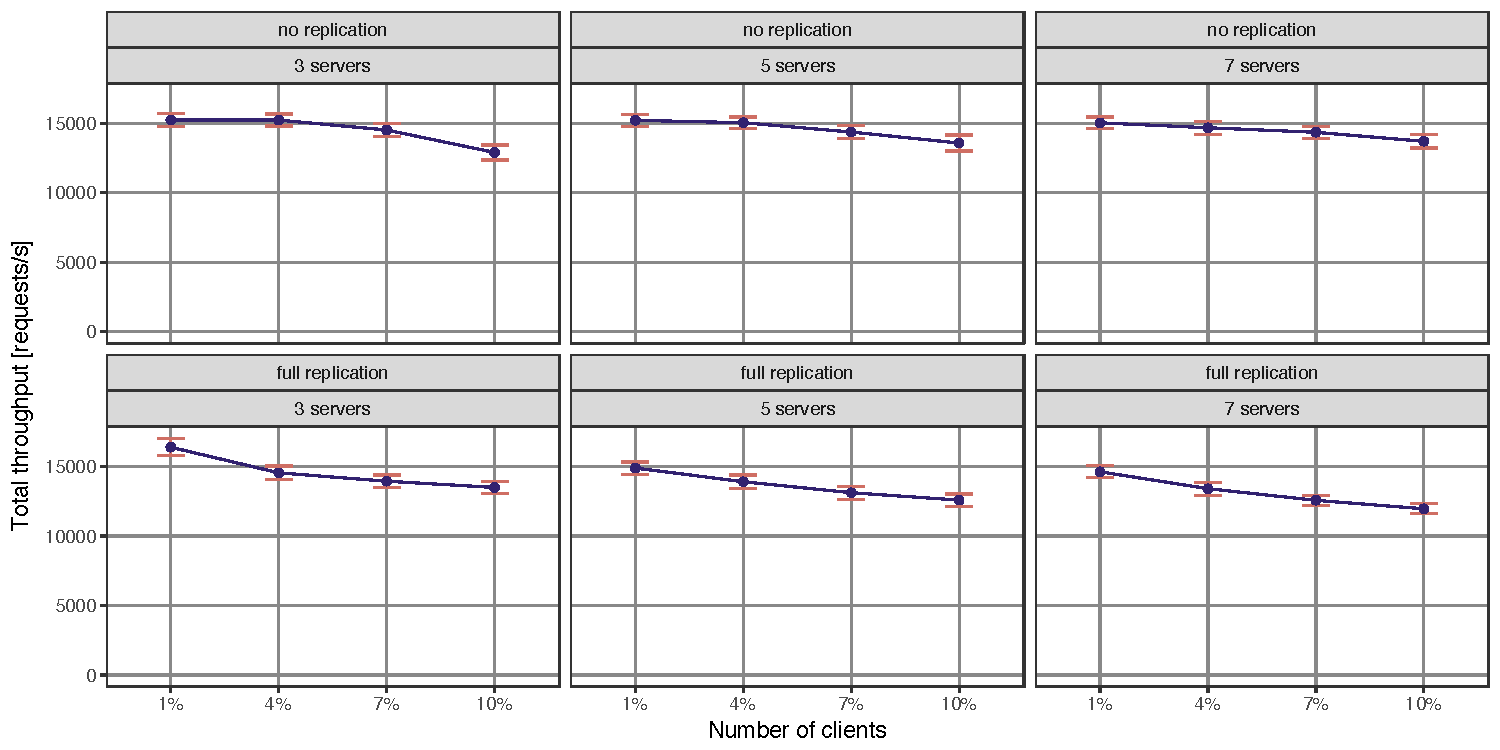
\includegraphics[width=\textwidth]{../results/writes/graphs/throughput_vs_writes.pdf}
\caption{Throughput of SUT as a function of $W$, for different values of $S$ and $R$. The line and points show the mean response time; red errorbars show the 95\% confidence interval over 10-second samples in a double-tailed t-test.}
\label{fig:exp3:res:throughput}
\end{figure}

\begin{figure}[h]
\centering
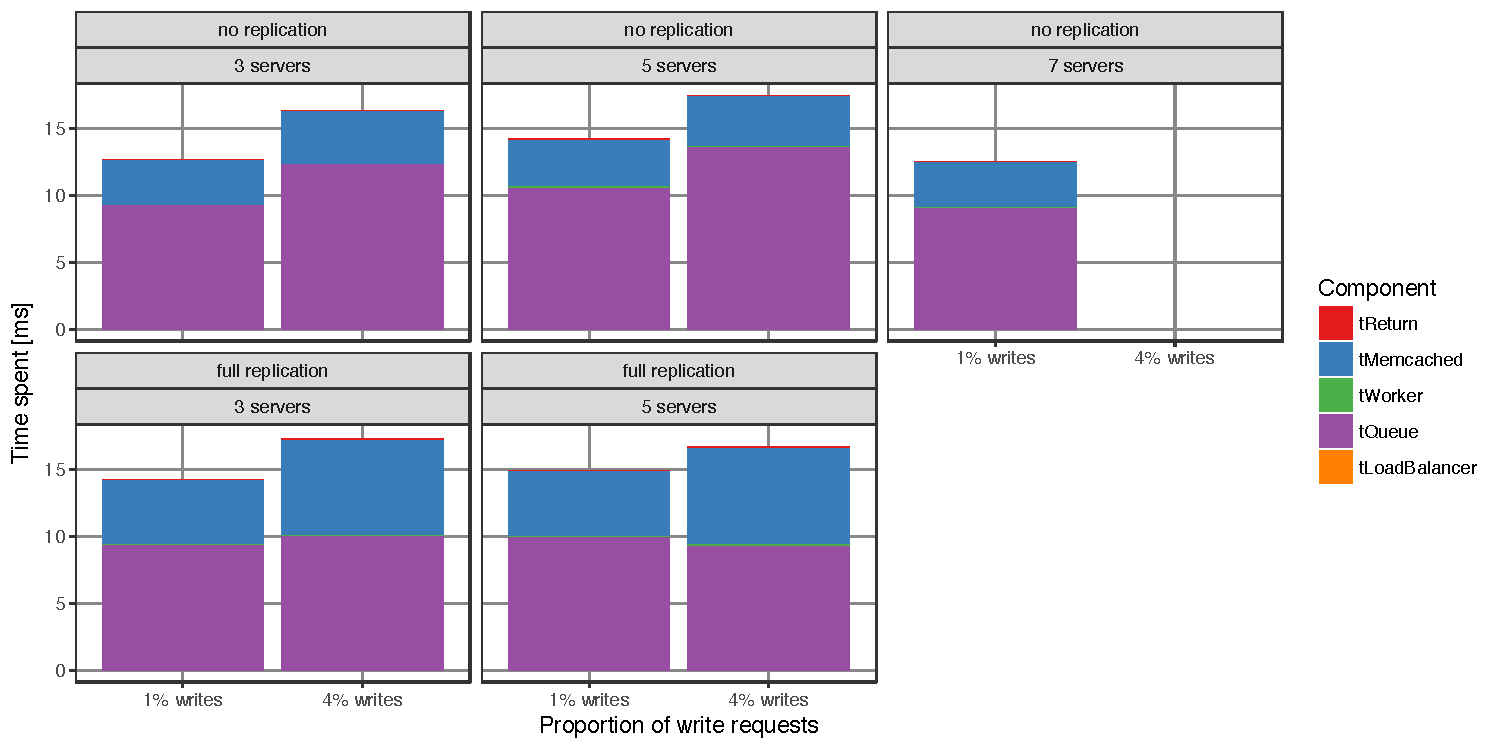
\includegraphics[width=\textwidth]{../results/writes/graphs/time_breakdown_vs_writes_set_abs.pdf}
\caption{Absolute cost of operations inside SUT, for different values of $S$ and $R$. Each column is divided into sections by the \emph{average} time spent in the respective component of SUT.}
\label{fig:exp3:res:breakdown:set:abs}
\end{figure}

\begin{figure}[h]
\centering
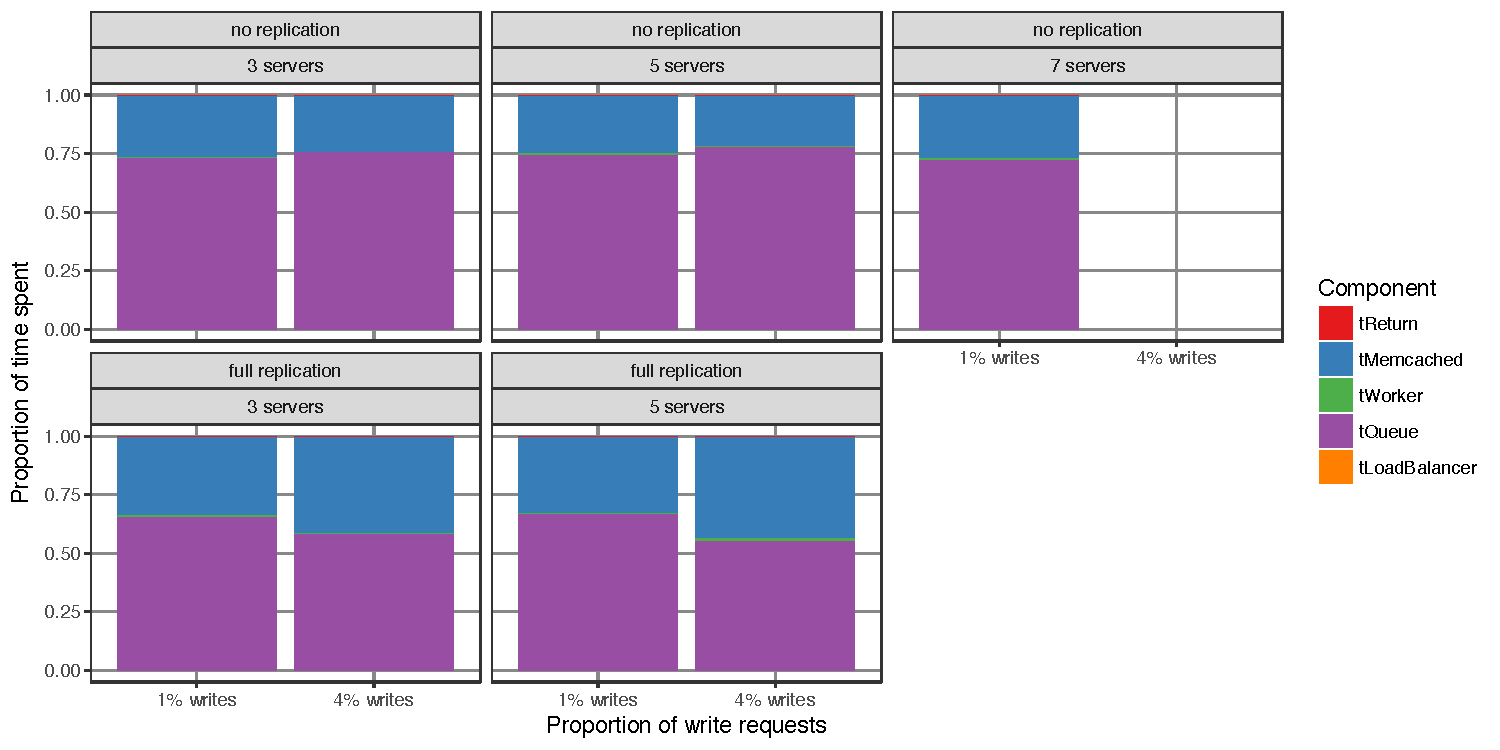
\includegraphics[width=\textwidth]{../results/writes/graphs/time_breakdown_vs_writes_set_rel.pdf}
\caption{Relative cost of operations inside SUT, for different values of $S$ and $R$. Each column is divided into sections by the \emph{average} time spent in the respective component of SUT, and then normalised to 100\%.}
\label{fig:exp3:res:breakdown:set:rel}
\end{figure}


\clearpage

\section*{Log file listing}
\addcontentsline{toc}{section}{Log file listing}

Each experiment's logs are compressed into a respective \verb+compressed.zip+ file and should be extracted to the directory where the \verb+.zip+ file is located. Each location mentioned in the table below is a directory that contains the middleware log (\verb+main.log+), the request log (\verb+request.log+) and memaslap outputs (\verb+memaslap*.out+). \\

\begin{tabular}{|c|l|}
\hline \textbf{Short name}& \textbf{Location} \\ 
\hline throughput-C*-T*-r* & \href{https://gitlab.inf.ethz.ch/pungast/asl-fall16-project/blob/master/results/throughput}{gitlab.inf.ethz.ch/.../results/throughput/clients*\_threads*\_rep*} \\ 
\hline replication-S*-R*-r* & \href{https://gitlab.inf.ethz.ch/pungast/asl-fall16-project/blob/master/results/replication}{gitlab.inf.ethz.ch/.../results/replication/S*\_R*\_rep*} \\ 
\hline writes-S*-R*-W*-r* & \href{https://gitlab.inf.ethz.ch/pungast/asl-fall16-project/blob/master/results/writes}{gitlab.inf.ethz.ch/.../results/writes/S*\_R*\_writes*\_rep*} \\ 
\hline 
\end{tabular} 
 
\end{document}